% !TEX root = ../main.tex
% Draft 10 describes the V7g design and checked source interfaces, not registered experimental performance.
% Source pointers and final-configuration TBDs: notes/DRAFT10_REVISION.md.
\section{Method}
\label{sec:method}
\sys\ connects visual target grounding to contact-aware action refinement. Attention-based Target Segmentation (ATS)
extracts target geometry; a Hidden-state Sub-task Recognition (HSR) probe helps maintain its identity across phases;
Link-specific Target Exemption (LTE) converts it into distance queries for individual links. Constrained Chunk
Refinement (CCR) applies those queries to the executed action horizon. Figure~\ref{fig:overview} summarizes the data flow.

% F02: Draft 10 conceptual data flow; separate serving and extraction passes are explicit.
\begin{figure*}[t]
\centering
\begin{tikzpicture}[
  x=1cm,y=1cm,font=\scriptsize,>={Stealth[length=1.6mm]},
  box/.style={draw,rounded corners=1.5pt,align=center,inner sep=3pt,text width=23mm,minimum height=9mm},
  pol/.style={box,fill=blue!8}, geo/.style={box,fill=green!9},
  tgt/.style={box,fill=orange!14}, opt/.style={box,fill=violet!10},
  every path/.style={line width=0.5pt}]
\node[box] (obs) at (0,3) {RGB + instruction\\+ proprioception};
\node[pol] (pi) at (3.3,3) {Frozen VLA\\serving pass};
\node[pol] (chunk) at (6.6,3) {Nominal\\action chunk};
\node[opt] (sqp) at (9.9,3) {\textbf{CCR}\\executed-horizon SQP};
\node[opt] (gate) at (13.2,3) {Post-check + gate\\execute / hold};
\node[pol] (extract) at (3.3,1.4) {Same checkpoint\\additional extraction pass};
\node[tgt] (ats) at (6.6,1.4) {\textbf{ATS}\\attention + 3D geometry};
\node[tgt] (lte) at (9.9,1.4) {\textbf{LTE}\\link-specific queries};
\node[tgt] (grasp) at (13.2,1.4) {Grasp state\\attached geometry};
\node[box] (depth) at (0,-0.4) {Calibrated depth\\+ capture state};
\node[tgt] (hsr) at (3.3,-0.4) {\textbf{HSR}\\trained linear probe};
\node[geo] (field) at (6.6,-0.4) {Self-filtered depth\\TSDF / ESDF};
\draw[->] (obs)--(pi); \draw[->] (pi)--(chunk); \draw[->] (chunk)--(sqp); \draw[->] (sqp)--(gate);
\draw[->] (obs.south) |- (extract.west);
\draw[->] (extract)--node[above,font=\tiny]{attention}(ats);
\draw[->] (extract)--node[right,font=\tiny]{prefix features}(hsr);
\draw[->] (hsr.east)--(4.9,-0.4)--(4.9,0.7)--([xshift=-7mm]ats.south);
\draw[->] (ats)--node[above,font=\tiny]{target}(lte);
\draw[->] (ats.north)--(6.6,2.15)--node[above,font=\tiny]{target geometry}(13.2,2.15)--(grasp.north);
\draw[->] (depth.south)--(0,-1.2)--(6.6,-1.2)--(field.south);
\draw[->] (depth.north)--(0,0.45)--(5.45,0.45)--([xshift=-11mm]ats.south);
\draw[->] (field.east)-|(lte.south);
\draw[->] (lte)--(sqp);
\draw[->] (grasp)--(lte);
\draw[->,dashed] (gate)--node[right,font=\tiny,align=left]{execution\\feedback}(grasp);
\end{tikzpicture}
\caption{\textbf{System overview.} The VLA serving pass produces the nominal chunk. A separate pass of the same frozen
checkpoint supplies attention for ATS and cached features for the trained HSR probe. Target geometry, phase-dependent
identity updates, and grasp state configure the link-specific queries used by CCR. Dashed feedback denotes recorded
execution information. The diagram describes the method, not measured performance.}
\label{fig:overview}
\end{figure*}


\subsection{Task-conditioned geometric constraints}
\label{sec:overview}
At request $t$, a frozen VLA receives RGB images, proprioception, and an instruction $l$, denoted by $(o_t,l)$, and
predicts an action chunk $A_t=\pi_\theta(o_t,l)$. Only its first $K$ of $H$ rows will be executed before replanning.
We refine the arm-joint references $Q^{\mathrm{ref}}\in\mathbb{R}^{K\times n_q}$ in those rows; gripper commands and
the remaining rows are passed through unchanged. Calibrated depth is an additional input to the geometric layer.
The active manipulator and its contact-link set $\mathcal L$ are supplied to the system.

Let $\mathcal T_t$ denote the observed target geometry, $s_t$ the inferred sub-task, and $z_t$ the grasp state.
Together they determine a distance query $\delta_{i,t}$ for each modeled robot or attached-object sphere $i$.
For center $c_i(q_k)$, radius $r_i$, and margin $m_{ik}$, we define
\begin{equation}
h_{ik}(Q)=\delta_{i,t}\big(c_i(q_k)\big)-r_i-m_{ik}.
\label{eq:clearance}
\end{equation}
Refinement seeks a trajectory close to the VLA reference while satisfying these modeled clearance constraints and
joint limits. The key dependence is in $\delta_{i,t}$: the same surface can be permitted for a contact link, retained
for another link, or represented as an attached object. Sections~\ref{sec:grounding}--\ref{sec:exemption} construct this
dependence; Sec.~\ref{sec:refine} describes the optimizer.

\subsection{From VLA attention to target geometry}
\label{sec:grounding}
An attention peak indicates a candidate location, but does not provide the object's full 3D extent. Conversely,
geometric clustering separates spatial regions without identifying which one the policy is manipulating. ATS combines
these signals by using attention to seed and rank geometric regions (Fig.~\ref{fig:fig03_attention_to_3d}).

\paragraph{Attention and multi-view lifting.}
For each camera $v$, we read an action-to-image attention map $\alpha_t^v$ from a fixed layer and head at the first
denoising step. The current implementation uses layer~8, head~2, and the last action-token query, producing a
$16\times16$ map for each of three views. An instrumented copy of the same frozen checkpoint performs an additional
prefix and first-denoising-step pass; it is separate from the pass serving actions. HSR reuses the prefix cache of
this extraction pass. \tbd{Document the attention-head selection data and its separation from final evaluation.}

We upsample $\alpha_t^v$ into the depth image coordinates. A valid pixel $u$ with depth $D_t^v(u)$ is lifted by
\begin{equation}
x_t^v(u)=T_t^v\!\left[D_t^v(u)(K^v)^{-1}\widetilde u\right],
\label{eq:lift}
\end{equation}
where $K^v$ is the camera intrinsic matrix and $T_t^v$ maps camera coordinates to the robot base at capture time.
Robot observations are self-filtered. The resulting points are fused on a voxel grid, retaining the maximum
attention value of observations within each voxel and then rescaling the fused attention by percentiles.
Low attention does not remove geometry from the scene map.

\paragraph{Geometric extent and target selection.}
We fit support planes and take high-attention, non-support points as seeds. Density-based clustering~\cite{ester1996dbscan}
grows candidate regions using the full non-support cloud, including low-attention points. Candidates are ranked by
their mean attention, compactness, and proximity to the attention peak. We filter candidates using gripper aperture,
support height, and a persistent destination estimate. In the current pick-and-place implementation, a persistent
high-ranked non-graspable cluster supplies the destination estimate. This is a geometric heuristic, not a general
semantic recognizer of receptacles.

The selected cluster supplies $\mathcal T_t$. A competing identity must persist across requests before replacing it;
during grasp approach and closure, switching additionally requires evidence that the old target is lost and the hand
has moved away. We retain the pre-closing geometry during closure to reduce shrinkage from finger occlusion. This
geometry is an estimate of the observed object, not a completed model of its unseen surface. A geometrically merged
target and obstacle can therefore produce an incorrect exemption; the evaluation must measure extent quality as
well as identity accuracy.

\begin{figure*}[t]
\centering
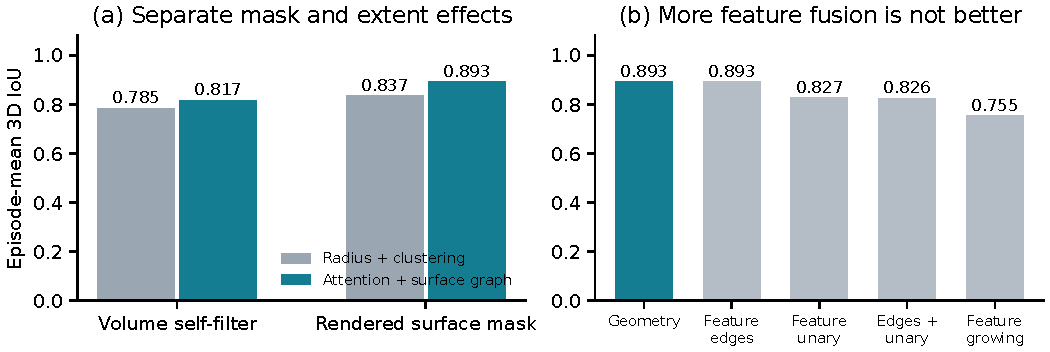
\includegraphics[width=\textwidth]{../figures/ifg_results/results.pdf}
\caption{\textbf{Measured development evidence.}
(a) The rendered robot mask improves both methods; the proposed extent pipeline retains an advantage when the mask is matched.
(b) With that improved geometry fixed, prefix-layer-8 feature edges leave IoU nearly unchanged, while prototype unaries and feature-conditioned growing reduce it.
All bars show episode-mean observed-surface IoU over 32 development episodes; they do not report held-out segmentation or physical safety.}
\label{fig:fig03_attention_to_3d}
\end{figure*}


\subsection{Maintaining the target across manipulation phases}
\label{sec:phase}
Target identity and physical attachment require different signals. HSR supplies a coarse phase for controlling
identity updates; a grasp state machine uses executed gripper commands, measured opening, and geometric evidence to
determine attachment and detachment.

\paragraph{A trained probe on frozen features.}
Let $\mathcal V_t$ be the value vectors at layer~4, key-value head~0 of the extraction pass. We concatenate means over
valid text tokens and image tokens into a feature $f_t\in\mathbb R^{512}$ and predict
\begin{equation}
p_t=\operatorname{softmax}\!\left(W\frac{f_t-\mu}{\sigma}+b\right).
\label{eq:probe}
\end{equation}
The normalization and linear classifier are fitted using phase annotations from the embodiment demonstrations,
with VLA weights held fixed. Text-token features include the instruction and tokenized state. The three classes are
\emph{pick}, \emph{place}, and \emph{home}; \emph{home} denotes post-release retreat and return. The predicted label is
confirmed over three consecutive requests. This is supervised probe training, not additional VLA training for
collision avoidance. \tbd{Finalize the probe training/validation split and phase-label specification in Appendix C.}

\paragraph{Phase and grasp-state roles.}
The confirmed phase controls target adoption and switching as in Table~\ref{tab:subtask}. It does not directly turn an
object into attached geometry. A retained target may still allow grasp contact while the phase has already changed
to \emph{place} but the grasp is unconfirmed. Once the grasp state is \textsc{held}, the representation changes as
described below. Release or detected slip detaches the object; a subsequent confirmed \emph{home} label clears the
retained target identity after \textsc{placed} has been observed. This distinction prevents phase predictions from
being treated as physical grasp measurements.

\begin{table}[t]
\centering\small
\begin{tabularx}{\columnwidth}{@{}l>{\raggedright\arraybackslash}X@{}}
\toprule
Confirmed phase & Target-identity rule \\
\midrule
\emph{pick} & Permit candidate adoption and persistent switching. \\
\emph{place} & Block new adoption and switching; retain the current identity. \\
\emph{home} & Block adoption/switching; clear the identity after \textsc{placed}. \\
\bottomrule
\end{tabularx}
\caption{HSR gates target identity. Before a label is confirmed, the underlying geometric selection rules apply.
Attachment and detachment are controlled separately by the grasp state.}
\label{tab:subtask}
\end{table}

\subsection{Link-specific contact and attached geometry}
\label{sec:exemption}
\paragraph{Scene distance field.}
Self-filtered depth is integrated into a TSDF and converted to an ESDF with the cuRobo mapper~\cite{sundaralingam2026curobov2}.
The scene distance $d_t$ combines coarse coverage with a finer window around the hand's swept region. The target
remains in this scene field before attachment. Unobserved space is treated as free by the current implementation;
therefore the constraints concern reconstructed surfaces.

\paragraph{A separate query for contact links.}
When a target is retained and no object is attached, LTE constructs a second fine ESDF by removing seed voxels in a
ball fitted to $\mathcal T_t$, padded by one voxel and clipped above the support plane. This does not alter the scene
field queried by other links. Let $f_t(x)$ be the target-excluded fine field, $\mathcal W_t$ its spatial window, and
$b_t(x)$ the distance to that window's boundary. The implemented query is
\begin{equation}
\dfree_t(x)=
\begin{cases}
\min\{f_t(x),\max\{d_t(x),b_t(x)\}\}, & x\in\mathcal W_t,\\
d_t(x), & \text{otherwise}.
\end{cases}
\label{eq:exempt}
\end{equation}
The boundary term accounts for the limited extent of the fine field. Defining $e_t=1$ when this exception is active,
the robot-link queries are
\begin{equation}
\delta_{i,t}(x)=
\begin{cases}
\dfree_t(x), & i\in\mathcal L\ \text{and}\ e_t=1,\\
d_t(x), & \text{otherwise}.
\end{cases}
\label{eq:linkquery}
\end{equation}
Here $\mathcal L$ contains the palm and fingers of the supplied active hand. Thus the exception is specific to a
geometric region and a link set. Because the removed region approximates the target with a ball, nearby surfaces
inside that region may also be removed from the contact-link field. The unmodified scene field remains available
to non-contact links; selectivity within the excluded region depends on target geometry quality.

\paragraph{From scene object to attached object.}
On a confirmed grasp, pre-closing target points are transformed into the palm frame and approximated by attached
query spheres. The observed body estimate is used to limit sphere size and offset. Its volume is cleared from the
environment map to avoid counting the object as an obstacle to itself, and its moving spheres query the remaining
environment with a destination clearance term. Attachment therefore changes both sides of the collision query:
the object leaves the environment representation and joins the moving geometry. After detachment, subsequent depth
observations reintroduce it into the scene. The fitted spheres approximate observed extent; coverage of the true
object must be checked for the shapes used in evaluation.

\subsection{Refining and checking the executed chunk}
\label{sec:refine}
CCR uses sequential quadratic programming (SQP) over the executed horizon. Its trajectory objective is
\begin{equation}
\begin{aligned}
J(Q)={}&w_{\mathrm t}\|Q-Q^{\mathrm{ref}}\|_F^2
       +w_{\mathrm s}\|\Delta^2Q\|_F^2\\
      &+w_{\mathrm c}\|Q_{\mathcal O}-\bar Q^{\mathrm{prev}}_{\mathcal O}\|_F^2,
\end{aligned}
\label{eq:qp}
\end{equation}
where $\mathcal O$ is the available overlap with the previous chunk shifted according to execution feedback.
With execution feedback enabled, invalid or unexecuted history is omitted. At iterate $Q^j$, clearance constraints are
linearized as
\begin{equation}
h_{ik}(Q^j)+\langle\nabla h_{ik}(Q^j),Q-Q^j\rangle_F+\xi_{ik}\ge\beta,
\label{eq:linearized}
\end{equation}
where $\langle\cdot,\cdot\rangle_F$ is the Frobenius inner product and $\beta$ is a clearance buffer, with nonnegative
slack $\xi$ penalized by $w_{\xi}\|\xi\|_1$. Each QP includes joint-position bounds, softened velocity
and acceleration bounds, and a trust region, and is solved with OSQP~\cite{stellato2020osqp}. A subset of low-clearance
rows enters the QP; the candidate is subsequently checked against all configured rows at the command waypoints.
Slack-assisted optimization does not itself establish feasibility.

\paragraph{Execution gate.}
The execution gate combines the post-check, field validity, and solver status. A rejected chunk holds the arm at
its measured pose while preserving the gripper command. The current implementation also has a collision-only
fallback: a refined chunk may be accepted when modeled spheres are nonpenetrating and its minimum clearance is no
worse than at the current pose, even if a positive margin is unmet. \tbd{Freeze the final gate configuration and report
fallback use separately in Appendix D.} These checks apply to the configured query geometry and sampled waypoints;
they are not a continuous-time or whole-body safety guarantee.

\paragraph{Implementation scope.}
We instantiate the layer with an embodiment-fine-tuned $\pi_{0.5}$, two 7-DoF arms, and two gripper channels
($H=50$, $K=8$). The client executes commands at 15\,Hz, giving a nominal chunk duration of 533\,ms; this is a timing
budget, not a measured system latency. The present collision queries cover gripper links and attached-object
approximations, with self-collision disabled. ATS thresholds, field resolutions, query geometry, probe fitting, and
solver settings belong in the implementation appendix. \tbd{Finalize the experiment snapshot and Appendix B--D
settings; measure the complete policy, extraction, geometry, refinement, and communication cost.}
